% File project.tex
%% Style files for ACL 2021
\documentclass[11pt,a4paper]{article}
\usepackage[hyperref]{acl2021}
\usepackage{times}
\usepackage{booktabs}
\usepackage{todonotes}
\usepackage{latexsym}
\renewcommand{\UrlFont}{\ttfamily\small}
\usepackage{multirow}

% This is not strictly necessary, and may be commented out,
% but it will improve the layout of the manuscript,
% and will typically save some space.
\usepackage{microtype}

\aclfinalcopy 

\newcommand\BibTeX{B\textsc{ib}\TeX}
\usepackage{amsmath}

\DeclareMathOperator*{\argmax}{arg\,max}
\DeclareMathOperator*{\argmin}{arg\,min}

\title{11-777 Spring 2021 Class Project\\
Analysis of Baselines}

\author{
  Christian Deverall\thanks{\hspace{4pt}Everyone Contributed Equally -- Alphabetical order} \hspace{2em} Jingyuan Li $^*$ \hspace{2em} Artidoro Pagnoni $^*$ \\
  \texttt{\{cdeveral, jingyua4, apagnoni\}@andrew.cmu.edu}
  }

\date{}

\begin{document}
\maketitle

% sections: High level (explain seen vs unseen),  Segmentation, Action-level 

\section{Introduction}

After performing an analysis of the two baselines ``Modular Object-Centric Approach'' (MOCA) \citep{singh2020moca} model and  ``Sequence-to-Sequence with Progress Monitor'' model (baseline of the ALFRED proposal paper) \citep{ALFRED20}, we identify some areas that could lead to performance improvements. In this report we explain in detail what specific limitations were of greatest interest to our team, in the context of a multimodal machine learning class, and how we plan to mitigate these limitations for the MOCA model. 

\section{Motivation and Challenges}
In the ALFRED world, actions are not always valid. This might be due to a variety of reasons, for example, objects could be blocking the movement of the agent, or an object the agent wants to interact with might not be present in the image.   
In the previous report, we computed statistics on the cause for an action to be invalid for the MOCA model (statistics reported in Table \ref{tab:error_analysis}).
Our main observation was that in both seen and unseen scenes that majority of invalid actions are due to two categories: the agent is unable to move (blocked) and the object is visible but not located correctly by the interaction mask. 

We also observed that 28\% and 40\% (for seen and unseen scenes respectively) of trajectories are interrupted because they reach the limit of 10 errors. This indicates that the presence of many invalid actions causes a large portion of failures. The two major areas for improvement in this direction are: 1. spatial detection of the validity of an action and 2. visual detection of objects for improved interaction validity.

Based on these observations, we identify modeling action feasibility as an interesting avenue for performance improvement. This direction is particularly challenging in the context of Seq2Seq models such as those that have been employed in the ALFRED task. It is not trivial to train a Seq2Seq model that follows a golden trajectory and expect it to learn about the feasibility of actions in the ALFRED environments. The training paths don't involve any examples of actions that are not feasible. The agent is only provided with indirect information about action feasibility: it is guaranteed that all actions in the training trajectories are feasible and has to deduce by lack of examples including some actions that they are not feasible. Solving this challenge will be the primary focus of our work.

One overly naive approach to solve the problem is to simply decouple the action feasibility model and the action prediction model. Intuitively, a unimodal model that only uses visual cues could determine the feasibility of certain actions in a given space. This unimodal model could be used in combination with the action prediction component and ensure the most likely action that is feasible is chosen. However, this approach does not help the model obtain a better grounding of language and vision and become better at navigating its world. In our proposed approach, we do recommend using such module at inference time to avoid performing infeasible actions but we will focus on improving the Seq2Seq action prediction model itself.

Furthermore, we find that improving the modeling of action feasibility is most interesting in the multimodal context of the ALFRED task. In particular, by better understanding the feasibility of actions in relation to both language and vision cues, we believe that the agent might be able to better generalize its understanding to unseen environments especially. For example, in the instruction ``walk along the kitchen counter'', the agent might understand that the use of ``walking along'' generally indicates that there is an object that cannot be traversed next to it which in this case is the ``kitchen counter''. On one hand this allows the agent to better understand the semantic of the instructions, but also hopefully allows the agent to generalize its understanding of action feasibility to unknown objects. If in an unseen environment an instruction requires the agent to ``walk along the sofa'', by association to the training example of the kitchen counter, the agent would learn about the feasibility of walking into the sofa.

In summary, we believe that modeling action feasibility could both help improve performance by, among other things, providing a better grounding of the language instructions in the context of the multimodal ALFRED task.


\begin{table*}[]
\centering

\begin{tabular}{|l|c|c|c|c|}
\hline
                                             & \multicolumn{2}{c|}{Seen} & \multicolumn{2}{c|}{Unseen} \\ \hline
                                             & Failure     & Success     & Failure      & Success      \\ \hline
Agent blocked                                & 1514        & 139         & 2639         & 7            \\ \hline
Agent state not allowed                      & 127         & 2           & 79           & 0            \\ \hline
Object visible but not located correctly     & 1569        & 28          & 2191         & 3            \\ \hline
Object not found in scene                    & 96          & 0           & 202          & 4            \\ \hline
Object property not allowed                  & 170         & 9           & 102          & 2            \\ \hline
Others                                       & 163         & 0           & 124          & 0            \\ \hline
Target state not allowed                     & 105         & 0           & 46           & 0            \\ \hline
No valid target                              & 40          & 0           & 25           & 0            \\ \hline
Object not visible                           & 109         & 3           & 153          & 0            \\ \hline
Object state not allowed                     & 21          & 0           & 18           & 2            \\ \hline
                                             &             &             &              &              \\ \hline
Frequency of error limit (10 errors) reached & 0.28        &             & 0.40         &              \\ \hline
Number of Errors (when less then 10 errors)  & 4.44        &             & 4.91         &              \\ \hline
Average number of errors                     & 6.03        & 1.05        & 6.99         & 0.78         \\ \hline
Average length of sequences of errors        & 2.954       & 1.19        & 3.57         & 1.17         \\ \hline
\end{tabular}
\caption{Analysis of types of error messages returned by Thor for invalid actions. We compare failed and successful tasks as well as unseen and seen scenes. The first part of the table contains counts of errors of different types across the validation dataset. The second part computes statistics about the number of errors per trajectory.}
\label{tab:error_analysis}
\end{table*}

\section{Approach}
The proposed approach involves improving the model's understanding of its surrounding, in particular, its understanding of the feasibility of actions. We also propose two other approaches which are meant to improve the quality of the predicted mask which was one of the sources of action infeasibility.

\subsection{Action Feasibility Module}


\subsubsection{Action Feasibility Auxiliary Prediction}
Along with predicting the next action in MOCA, we propose an auxiliary prediction task. The model will predict which actions are feasible at each time step along the golden trajectories provided in the training set. 
We will gather the data on which actions are feasible at each time step of the golden trajectories by querying the simulator offline before training. 
The current prediction task only requires the agent to predict the next best action to undertake  and does not provide any clue to the model about any other differences in the available actions. Our hypothesis is that with the auxiliary action feasibility prediction task, the agent would develop an understanding of the available actions beyond whether they are the best next step: some of them are feasible and some are not.

To achieve this goal, we define an auxiliary loss function that tells the agent about feasible and infeasible actions. In specific, in the Action Policy Module of MOCA, we add an extra linear layer before the action output, denoted as $\hat{A}$, representing the feasibility of the action. We want the agent to learn from the environment which action is feasible in each time step. And each element in $\hat{A}$ is activated by sigmoid function $\sigma$. We train this additional layer using focal loss \cite{lin2017focal}:

\begin{equation}
\begin{split}
    & Loss = -\frac{1}{n_a} \sum_{i=1}^{n_a} a^{i} (1 - \hat{a}^{i})^{\gamma} log (\hat{a}^{i}) \\
    & + (1 - a^{i}) \hat{a}^{i}^{\gamma} log (1 - \hat{a}^{i})
\end{split}
\end{equation}

where $\gamma$ is a tunable parameter. Here we use focal loss instead of conventional binary cross entropy loss because most actions are feasible and only a minority of actions are not feasible. Focal loss helps reduce the influence of imbalanced samples.

% Why this is multimodal: Intuitively, the loss function above not only stresses the infeasibility of actions but also stresses the optimal actions. The optimal actions are informed by both the high-level instruction (eventual goal), and the low-level instruction (short-term goal), which is thus influenced by multi-modal data. Hopefully, the model will learn a better alignment between language, image, and its understanding of what can be done in the world.


\subsubsection{Action Feasibility Mask}
We propose a second stand-alone model that only uses the visual input and the interaction mask to predict the feasibility of an action. This model can be trained in a supervised fashion using the simulator sampling different locations and querying the feasibility of actions at those locations. 

Since the second model requires only visual input and action feasibility output, not depending on the previous step, the model can be trained offline. To train this model, we need a group of images ${I_1, I_2, ..., I_t}$ pre-collected from the simulator, and the corresponding action feasibility labels ${F_1, F_2, ..., F_t}$ at the location where the corresponding images are collected. The action feasibility in $F_n$ is 1 if the action is either a feasible navigational action or a feasible interactive action that acts on any objects in $I_n$, otherwise, it's 0. Given a visual feature extractor (e.g. ResNet, DenseNet) $\Phi(\o=cdot)$, we assume the output in the last layer of the model to be $F_{logits}$ of size $n_a$, where $n_a$ is the number of action. $F_{logits}$ is the score of action feasibility without any activation functions (i.e. it's the output from a linear layer). Then we generate the eventual action feasibility mask using the element-wise sigmoid function $\sigma$, i.e.

\begin{equation}
    \hat{F} = \sigma(F_{logits})
\end{equation}

Then we use the binary cross-entropy loss on each action for calculating the loss function, i.e. 

\begin{equation}
    Loss = -\frac{1}{n_a} \sum^{n_a}_{i=0} F^i log (\hat{F}^i) + (1-F^i) log ((1-\hat{F}^i))
\end{equation}
where $F^i$ is the feasibility of the $i^{th}$ action. By optimizing this target, we are able to train a module to tell the action feasibility.

After the module being trained, we will be able to use it for better inference. In specific, given the action preference prediction given by the module to be $\hat{A}$, the initial strategy to select action is 

\begin{equation}
    a* = \argmax(\hat{A})  
\end{equation}

To avoid bad actions, we now select the target action though

\begin{equation}
    a* = \argmax(\hat{A}\odot\hat{F})
\end{equation}
where $\odot$ is element-wise multiplication.

\subsection{Improved Instruction Use}

The model architecture for the MOCA paper is provided in figure \ref{fig:sys_arch}. As can be observed, the Visual Perception Module does not receive input from the step-by-step instructions. Its input consists solely of the high-level goal statement, the image embedding and the previously predicted action. This omission could explain our finding that one of the most common sources of invalid actions is when ``the object is visible but not located correctly by the interaction mask''. As a result, the equation for $h_{t,m}$ would change to the following:

\begin{equation}

    h_{t,m} = LSTM_{m}([\hat{v}_{t,goal};\hat{x}_{t,goal};a_{t-1};\hat{x}_{t,instr}])

\end{equation}

where (similarly to the notation of the MOCA paper) [;] represents concatenation, $\hat{v}_{t,goal}$ represents the attended visual features, $\hat{x}_{t,goal}$ represents the attended features for the high-level goal, $;a_{t-1}$ represents the previously predicted action and $\hat{x}_{t,instr}$ represents the attended features for the step-by-step instruction. 

\begin{figure*}
    \centering
    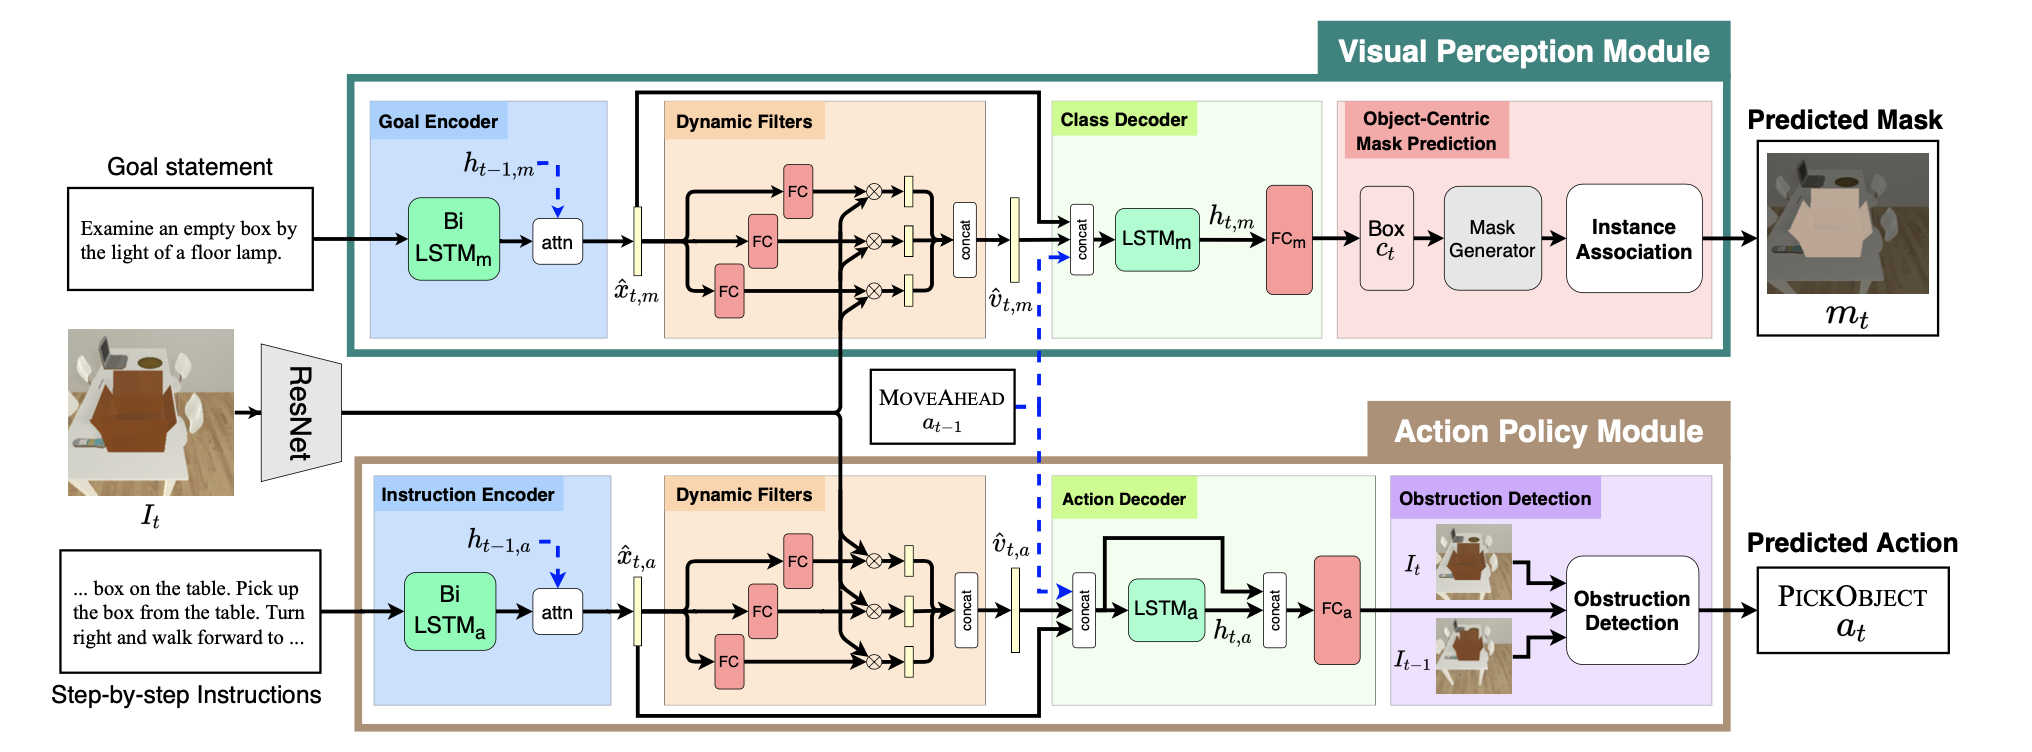
\includegraphics[width=\linewidth]{Reports/5-Proposed-Approach/system_arch.png}
    \caption{Detailed model architecture from the MOCA paper.}
    \label{fig:sys_arch}
\end{figure*}

% \subsection{Improved Previous Step Mask Use}

\subsection{Condition on Action to Predict Mask}

In this subsection, we propose another strategy to reduce the amount of invalid actions caused by bad mask predictions. MOCA uses object-centric mask prediction whereby the first step is to predict the class of the object to interact with. Importantly, the current predicted action is not provided in target class prediction. This is a weakness because knowledge of what action to take would influence what object to act upon. Intuitively, one would be less likely to predict ``the fridge'' as the object if one knew the action was ``cut''. As a result, we will explore two methods of inputting the action to the mask prediction. For both methods, we would still use ``Instance Association in Time'' as defined in the MOCA paper. The first method is to concatenate the one-hot encoding of the action to the hidden state $h_{t,m}$ as below:

\begin{equation}
% \underset{x}{\operatorname{argmax}} 
    c_t = \argmax_{k} FC_{m}([h_{t,m}; a_{t}]),

\end{equation}

where $c_t$ is the predicted class, $h_{t,m}$ is the hidden state of the VPM and $a_t$ is the predicted action of the current time step. The second method we will explore is to input the current action to the LSTM that outputs the hidden state $h_{t,m}$. In this case, equation 6 would change to the following: 

\begin{equation}

    h_{t,m} = LSTM_{m}([\hat{v}_{t,goal};\hat{x}_{t,goal};a_{t-1};\hat{x}_{t,instr};a_{t}])

\end{equation}

We will experiment on both methods and use the method with the better test performance.

\section{Expected Difficulties and Proposed Mitigations}
The primary difficulties that we expect to encounter involve the collection of action feasibility data. It will be trivial to collect data about navigation actions that don't require interactions with other objections. However, for interactive actions, we would like to gather data about whether any object in the image could be used with an interactive action. For example, for the action ``toggle'' we would like to know if there is any object in the image that can be ``toggled''. We plan to use the simulator to extract a mask for all objects in an image and query the simulator to verify if the actions are valid with any of the objects in the image.

Another difficulty that we might encounter is that there might not be enough examples of infeasible actions along the training trajectories. One way in which we have already planned to mitigate this issue is by using focal loss \cite{lin2017focal}. This loss is similar to binary cross entropy but helps with class imbalance issues. In case this is not sufficient, we might have to sample additional trajectories that are semantically equivalent but that have more infeasible actions along their way (by infeasible actions we mean actions other than the golden actions at a given time step that are not feasible). This could be done by for example walking closer to objects that cannot be traversed but still reaching all stages of the training trajectory where the agent has to interact with an object.

\section{Conclusion}
We propose a novel approach to improve the agent's ability to model its surrounding in the ALFRED task. We focus on teaching the agent how it can interact with its environment. This is particularly challenging for Seq2Seq models currently employed in the ALFRED task. Our methodology should provide the model with a better understanding of the feasibility of actions without requiring a full on reinforcement learning set up. We train the model to learn about action feasibility through an auxiliary prediction task and sampling more data from the simulator at each given step of training trajectories. Along with this main approach, we also propose additional modifications to MOCA that should help reduce the overall number of infeasible actions taken by the agent. 



\clearpage
% Please use 
\bibliographystyle{acl_natbib}
\bibliography{references}

%\appendix



\end{document}
